\documentclass{sigchi}

% Load basic packages
\usepackage{balance}  % to better equalize the last page
\usepackage{graphics} % for EPS, load graphicx instead
\usepackage{times}    % comment if you want LaTeX's default font
\usepackage{url}      % llt: nicely formatted URLs
\usepackage{caption}
\usepackage{subcaption}
\usepackage{float}
\usepackage{pdfpages}

% llt: Define a global style for URLs, rather that the default one
\makeatletter
\def\url@leostyle{%
  \@ifundefined{selectfont}{\def\UrlFont{\sf}}{\def\UrlFont{\small\bf\ttfamily}}}
\makeatother
\urlstyle{leo}


% To make various LaTeX processors do the right thing with page size.
\def\pprw{8.5in}
\def\pprh{11in}
\special{papersize=\pprw,\pprh}
\setlength{\paperwidth}{\pprw}
\setlength{\paperheight}{\pprh}
\setlength{\pdfpagewidth}{\pprw}
\setlength{\pdfpageheight}{\pprh}

% Make sure hyperref comes last of your loaded packages,
% to give it a fighting chance of not being over-written,
% since its job is to redefine many LaTeX commands.
\usepackage[pdftex]{hyperref}
\hypersetup{
pdftitle={Approximator - A system for presence and interruptibility-sharing},
pdfauthor={Kristian S. M. Andersen, Anders Bech Mellson and Mads Daniel Christensen},
pdfkeywords={spce, gse, presence, awareness},
bookmarksnumbered,
pdfstartview={FitH},
colorlinks,
citecolor=black,
filecolor=black,
linkcolor=black,
urlcolor=black,
breaklinks=true,
}

% create a shortcut to typeset table headings
\newcommand\tabhead[1]{\small\textbf{#1}}


% End of preamble. Here it comes the document.
\begin{document}

\title{Approximator}
\subtitle{A system for presence and interruptibility-sharing}
\numberofauthors{3}
\author{
  \alignauthor Anders Bech Mellson\\
    \email{anbh@itu.dk}\\
  \alignauthor Kristian S. M. Andersen\\
    \email{ksma@itu.dk}\\
  \alignauthor Mads D. Christensen\\
    \email{mdch@itu.dk}\\
}

\maketitle

\begin{abstract}
This paper presents a practical approach on how to get user presence and interruptability information using only a standard laptop.
\end{abstract}

\keywords{
  Global Software Engineering, Presence Awareness, Interruptibility, Social Contracts of Human Interactions
}

\terms{
  Documentation, Theory
}

\section{Introduction}
Globalization is an economical and societal trend that has pushed industries to move from local to global markets.
Working in a global setting requires practitioners to work in distributed arrangements.

Paraphrasing Herbsleb \cite{herbsleb2007}, many of the mechanisms that work correctly in a co-located setting are absent or disrupted in a distributed arrangement.
Different approaches \cite{bly1993media} \cite{fogarty2004myvine} \cite{hincapie2011design} \cite{lai2003myteam} \cite{want1992active} have been investigated to improve the awareness of the working context that a member of a virtual team has; nonetheless, information like the presence of virtual team members, trivial in a co-located setting, represent an interesting open area of investigation.

One fundamental difference between a co-located arrangement and a distributed one is the lack of presence awareness.
The ability to assess how interruptible another person is, becomes very hard when you are not in the same room.
When you are in the near proximity of another person it is fairly easy to assess the interruptibility of that person.
We use the interruptibility assessment to facility behavior that we consider socially acceptable.
If you work in a distributed setting you are dependent on tool support from computer and communication systems to provide availability information about your co-workers.
Today these systems are largely unaware of the social contracts of human interactions.

Research by the Human Computer Interaction Institute at Carnegie Mellon University \cite{fogarty2005predicting} shows that you can detect the interruptibility of a person using sensor inputs.
In their research they find that you can predict interruptibility with sensor inputs at an accuracy of 68\%.
The researchers note that their results could ``motivate the development of systems that use these models to negotiate interruptions at socially appropriate times.''

We will build upon their research and be inspired by their models in a practical pursuit of a presence and interruptibility-sharing system.
The work presented in this paper represents two primary contributions.
First, we demonstrate an implementation of a presence and interruptibility-sharing system for global software engineers.
Second, we evaluate the system.
This is done with a test where we compare the accuracy of our availability prediction model againts the accuracy achieved by humans trying to predict availability.

\section{Related work}
Research on using technology to support awareness in a distributed setting has been going on since the early 90’s.
Some of the work \cite{bly1993media} \cite{gaver1992realizing} \cite{mantei1991experiences} tries to keep an instant audiovisual connection between workplaces.
This has the benefit that not only intentional communication is supported, but also social communication since the co-workers is always visible.
But the approach has some drawbacks.
Users can feel self-conscious about the image of themselves being broadcasted.
Not only that but keeping high quality media streams running all day can also be expensive since it consumes a large amount of bandwidth.

Distributed teams can use instant messaging (IM) applications to communicate.
Research on IM usage \cite{nardi2000interaction} \cite{handel2002chat} \cite{tang2001connexus} has shown that IM is not only used for chatting, it is also used to negotiate availability.
Most IM systems rely on the user manually setting their status or on simple activity data, such as mouse movement.
This does not always reflect the availability of the user.

Fogarty et al. has shown that sensors can be used to extract satisfying accuracy data about a user.
They have used this data to construct a statistical model \cite{fogarty2004examining}.
Later Fogarty et al. goes on to show that it is possible to construct a prediction model for human interruptibility based on simple hardware sensors that is as accurate as humans predicting interruptibility from a video recording of a person working \cite{fogarty2005predicting}.

Several systems have tried to build an awareness solution using sensors.
The earliest work dates back to the active badge system \cite{want1992active}.
A similar approach has been tried in the IM system MyTeam \cite{lai2003myteam}, where they use an active badge sensor in combination with the users computer activity.
This solution builds upon the premise that success of communications is having prior knowledge about the availability of others before initiating contact.
Lack of this information may explain why over 60\% of business phone calls fail to reach the intended party \cite{whittaker1995rethinking}.
MyTeam differs from other IM systems in that participants can get information about the availability of colleagues even if that person is not running the MyTeam client.
MyTeam uses photos on a colored background to indicate availability.
A drawback of the system is that it takes up a large portion of the users screen. It is also not possible to initiate communication directly from the MyTeam client.

A system that also uses sensors to determine availability is MyVine\cite{fogarty2004myvine}.
MyVine resembles MyTeam in the way that they both show availability, and also uses continuous values (e.g. 0-100) in means of showing this.
What differs the two systems, is MyVine’s use of holistic aggregated sensors (speech
detection, location information, computer activity, and calendar information) instead of just two sensors(active badge proximity and keyboard and mouse).
The two systems differs in two more ways.
One is that MyVine is symmetric, which means the user has to be online in order to see other users availability.
The other is that MyVine is an almost-always-on system, which allows the users to continuously be shown as available, despite not having to run in the foreground.
MyVine has a problem with misinterpretations of speech as an indication of being unavailable, while users has observed the speech as an indication of availability.

The SenSay context-aware mobile phone \cite{siewiorek2003sensay} use accelerometer, light, and microphone sensor inputs to determine the availability of the user.
The phone dynamically adapts it’s volume, vibration etc to match the user's current context.
A novel feature about the phone is that the caller can communicate the urgency of their call.
SenSay uses a decision module, which analyzes the sensor input to decide which state the phone should be in.
The system requires the user to carry additional sensors besides the phone, which is not ideal from a user perspective.

In \cite{hincapie2011design} Ramos et al. evaluates the design space of availability-sharing and introduces six new relevant design dimensions for evaluating availability-sharing systems: abstraction, presentation, information delivery, symmetry, obtrusiveness and temporal gradient.
Informed by the evaluation of other systems InterruptMe is presented.
InterruptMe uses implicit inputs from the user to present availability information.
However to get these inputs several external sensors are needed.
This makes the system unable to run on commodity laptops.

\section{Approximator}

Based on the related work we want to provide a practical user-centric approach to sharing presence and interruptibility information in a Computer Supported Cooperative Work (CSCW) setting.
Our solution is called Approximator.
To support this system we design and build an a scalable infrastructure that can be easily deployed with cloud services.
The infrastructure facilitates the presence and interrubtibility by reading raw sensor input and intepreting presence and interrubtibility from that.
Building on the research of Fogarty et al.\cite{fogarty2005predicting} we will predict interruptability from raw sensor input but only using sensors found in modern laptops. We will also evaluate the system in the same way to find whether Approximator can sustain the same 68\% precision rate.

\subsection{Overall System Architecture}

The central component of Approximator is the infrastructure.
The infrastructure is a server component that is deployed to a cloud service.
The infrastructure exposes a REST API that Sensors and Demonstrators use to communicate through.
Sensors register themselves with the infrastructure and sends raw sensors data.
The infrastructure aggregates and interprets the raw sensor data to deduct presence and interruptibility of users.
Demonstrators pull interpreted presence and interruptibility from the infrastructure to expose it to users.


\begin{figure}[H]
  \centering
  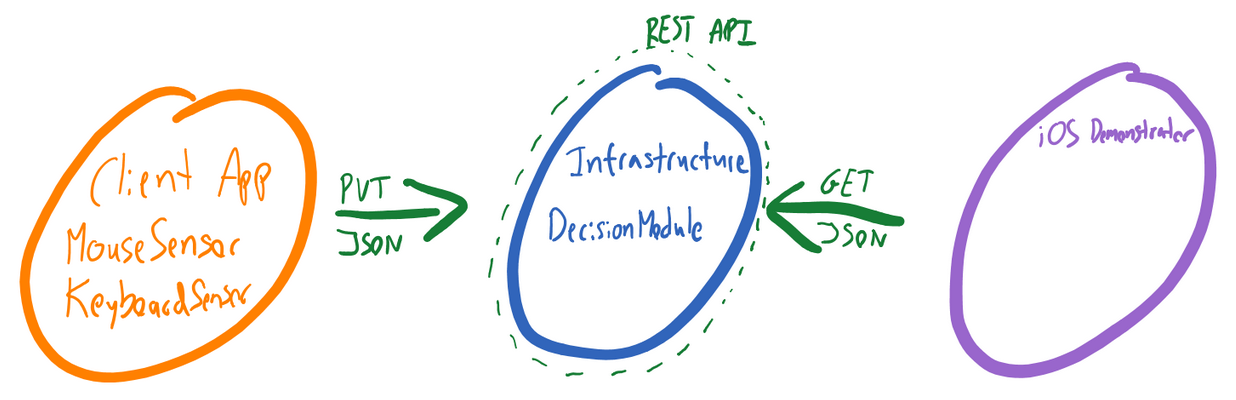
\includegraphics[width=\columnwidth]{figures/architecture.png}
  \caption{SKETCH!!! System architecture.}
  \label{fig:architecture}
\end{figure}

% The entire system is build around the infrastructure
% The Infrastructure lives in the cloud and is based on the actor model.
% Each sensor registers itself with the infrastructure and sends raw sensor data
% The infrastructure aggregates and interprets the data.
% Demonstrators poll presence and availability information from the infrastructure
% and present it to the users
% Data can be either polled/posted from/to the server or streamed
% Streams provide real-time updates in presence availabiltiy.
% This is possible because of the highly scalable infrastructure
% Where each User has a cluster of sensors nodes

\subsection{Infrastructure}
To provide presence and availability information to cloud workers we need a few things.
Firstly we need to gather data input from the working environment.
Secondly we need to aggregate this data and combine it for each user.
Lastly we need to look at the data and through analyzises provide presence and availability information.

All these tasks are combined in our infrastructure which can read input from sensors and analyze this with a decision module.

The work flow of the infrastructure is:
\begin{enumerate}
  \item Gather data
  \item Aggregate data
  \item Analyze data
  \item Provide data
\end{enumerate}

\subsubsection{Design}
The infrastructure is built to support many sensors for each user.
This modelling can lead to a very high amount of sensors connecting to the system.
To support this scalability need we base our system on the actor model by Carl Hewitt \cite{hewitt1973universal}.

Many software applications are written using the object oriented modelling.
The actor model is an alternative way to model computer programs.
In the actor model the unit of work is an actor.
In object oriented programming the unit of work is an object.
Actors communicate by sending messages to each other.
Actors does not share state, making it possible to run actors in parallel and even on different machines.
This makes the actor model a good candidate for building highly scalable applications.

There are several frameworks implementing the actor model, such as Akka \cite{akka}, Project Orleans \cite{orleans} and most famously Erlang \cite{erlang}.
For this project we have chosen Akka because it is Java based.
This supports the technical knowledge in our group.

We use the general programming language Scala \cite{scala} to program our Akka-based infrastructure.

It is possible to deploy Akka applications on a server which can run Java.
For this project we have chosen to deploy our system to Azure \cite{azure}, Microsoft's cloud service for developers.
Having the infrastructure running at a cloud provider makes it reachable from the standard internet.
This enables us to build sensors and demonstrators that can run anywhere, as long as they have an internet connection they can reach our infrastructure.

\subsubsection{Data}
Gathering data happens by sensors providing data.
To communicate with our infrastructure a sensor needs to register with the service.
When a sensor registers itself it provides a username.
This username is used to aggregate a group of sensors together around the notion of user.

\subsubsection{Decision Logic}
Raw sensor data does not say much about presence or availability.
We need to analyze the data to make sense of it.
The infrastructure has a decision module which can do this.

When a client asks the service to provide data the decision module translates the data before serving it through the REST API.

\subsection{Sensors}
To gather data about the users presence and availability we use sensors.
This project has restricted itself to only look at sensors which are available in commodity laptops.
Commodity laptops can be many things, we define it as a machine with the following sensing capabilities:
\begin{enumerate}
  \item Mouse
  \item Keyboard
  \item Microphone
  \item Lightsensor
  \item Operating System which supports running custom software
  \item Webcam
  \item Bluetooth
  \item Wifi
  \item More???
\end{enumerate}

Modern laptops are every pervasive system developers dream, filled with all kinds of sensors that can be used to sense the environment.
Every modenr laptop is equiped with sensors like microphones, webcameras, trackpads, keyboards and light sensors.
They also contain radios for Bluetooth, Wifi and Infrared.

% Something about modern laptops

% What sensors are available in a modern laptop?
% Which sensors should we use given Fogarty?
% Which sensors can we exclude?
% - Inputs
%	- Keyboard
%	- Mouse
%	- Microphone?
% Which sensors do we choose to include and how?
% Which sensors do we choose to exclude and why?
% Example: We exclude the webcam because Fogarty
% shows that it is not needed when they have the
% microphone

\subsubsection{Keyboard and Mouse}
By using the mouse and keyboard as sensors we collect every mouse movement and keyboard events and send last recorded activity every second.
With this information we can infer presence due to the fact that there is someone triggering these events.

The issue with using keyboard and mouse as sensors, is that even though they are a strong indicator of presence, we cannot decipher, based on these two sensors alone, who or what this presence is.
We can tie the machine to a specific user, but we can not infer if the machine is being used by a colleague or if a cat decide to rest on the keyboard.

Another issue with mouse and keyboard sensors is that they provide a very weak indicator of non-presence.
When a key is pressed or the mouse moved, we know that someone is interacting with the machine, but the lack of action cannot tell us whether a person is present or non-present.
A person could be talking on the phone, reading, watching a video etc. all in which the person is present, but the mouse and keyboard cannot provide us with this information.

In terms of interruptibility the information from the mouse and keyboard is too ambiguous to deduct whether a person is busy or interruptible.
If the identity of the person sitting in front of the computer could be confirmed, it would still be difficult to determine whether the behavior is an indication of interruptibility.
An approach to determine interruptibility based on these sensors, would involve sending all information to the decision logic, effectively acting as a key logger, and therefore raising security and privacy issues.
% Jeg ved ikke om det er noget vi skal gå i dybden med, eller om det er nok bare at nævne det her.... eller om det overhoved skal nævnes.
% Min overvejelse er om man kunne bruge en vægtet dictionary hvor specifikke ord fik en vægt på hvor arbejds releterede de er og evt kombinere det med en form for pattern matching hvor sprog mønstre blev undersøgt.
This approach will be described later in the decision logic section.

\subsubsection{Microphone}
The use of a microphone as a sensor allows Approximator to sense the presence of a person, even if the person is not directly interacting with the machine.
With more advanced speech recognition algorithms it could even be used to identify the person/persons speaking.
This would provide us not only with presence, but also identity, which was a problem with the keyboard and mouse sensors.

The same issue with the detection of non-presence also appears with the microphone, it is not possible to infer non-presence from the lack of sound.
As described with the keyboard and mouse sensors, a person can perform activities that does not trigger the sensor, and thus be present without detection.

Beside the detection of presence, the microphone provides a tool for inferring interruptibility.
According to Fogarty et al\cite{fogarty2005predicting} speaking present a situation of non-interruptibility.
\subsubsection{Lightsensor}
????

\subsubsection{Process monitor}
This sensor is slightly different than the others since it primary purpose is not to sense presence, but interruptibility.
The idea of the process monitor is to supply it with a list of processes (programs) that it should monitor.
This list consists both of work and leisure associated processes, and the process monitor report if any and which program are in the foreground. %and receiving user input.
Through this we obtain the same or weaker notion of presence and non-presence as we did with the keyboard and mouse sensor, but gain a stronger tool to infer interruptibility.

\subsubsection{Geolocation}
This sensor works by looking up the machines registered ip address, or if available uses the machines build-in gps, and uses this to acquire a geographical address.
Knowing the whereabouts of the machine neither infers presence nor interruptibility on its own.
But it does supply the other sensors and the decision module with useful information regarding the geographical setting of the machine.
The most simple use of this is to detect if the machine currently resides at the office, home, or another location.
But one of the more useful appliances would be in combination with the webcam.
If the webcam can detect action such as a person entering or leaving the room, this information could tells us whether the a person is in close proximity to the machine, but only that.
Combined with even the coarse location of the machine, Approximator could infer that a person was in a specific office, in close proximity the machine.

\subsubsection{Webcam}
Like the microphone the webcam enables Approximator to sense the presence of a person without the person having to interact with the machine, but differs in the way it does so.
In the setting of a room a microphone can sense if someone is in the room, but it is hard for the microphone to infer where in this room that they are located.

The webcam (based on the assumption that the webcam is facing the same way as the viewfield of the screen) can sense if someone is directly in front of the screen, which supplies a powerful indicator of presence, but also an indicator of non-presence.
Unlike the other sensors, the webcam can sense if a person is sitting in front of the machine, even if the person is not directly interacting with the machine.
But even though the webcam can infer non-presence, there are still some issues.
For example, if a person is located in his/her office but not facing the machine e.g. sitting in a chair across the office, the person will be present and possible available, but the webcam will not be able to detect a person but only movement.

The webcam can also apply face-recognition in order to determine the identity of the person present.
It could also be possible to detect actions that the person is executing e.g. entering the room leaving, leaving the room, reading a book etc. that can be used to measure interruptibility.
But of course for these things to work, the actions must be performed within the view-field of the webcam.

\subsubsection{Bluetooth, Wifi and Infrared}
These sensors can not be used to infer presence nor interruptibility on its own.
But they can be used to detect other devices such as mobile devices or beacons.
If we assume that a person always carries his/her mobile device with them, then the bluetooth or wifi beacon from this device can be used to infer if the persons proximity to the machine.
Another usage is if the office the person works in have beacons installed at the workplace, ether as Bluetooth or WiFi beacons, then the machine can infer its current symbolic location.
This can be used to infer presence by detecting if the mobile device is nearby.
The issue here is if the person should forget their mobile device, ether nearby the machine or at home.
In these cases the sensor would receive false data i.e. data that provides wrongful information regarding presence or interruptibility.


\subsection{Decision Logic}
While each sensor by itself does not provide useable information, we can actually get quite accurate reading by aggregating the sensors and feeding them into a decision module.
This section will provide information about how we approach this.

% - Screenshot of app with presence + interruptibility

\section{Evaluation}

\subsection{Methodology}
We applied the same methodology for evaluation as Fogarty et al \cite{fogarty2005predicting} where we used a video recording of a user in their work environment and had the user assess their interruptibility on 1 to 5 scale in specific sequences of the video.
Afterwards we presented the user to a confidence questionnaire, to test the users confidence in their own assessments.
We use this information to find the sequences in the video where the user is most confident and use these as base for our tests.

We have gathered test persons from our university grounds by inviting people through personal relations and facebook fora related to university activities.
We chose students from the university because it facilitated fast testing since the students were on campus and could easily participate in the study.
Then we showed the video to x test persons and asked them at specific situations in the video to which degree they found the user as interruptible or non-interruptible on a scale from 1 (non-interruptible) to 5 (interruptible)

Following we compared estimator-test-persons answers and the values that Approximator had calculated to the values had reported.
This was done by plotting the values into two confusion matrices.
One comparing the answers of user to answers of the test persons.
And one comparing the answers of the test persons to the results of Approximator.
By finding correlations between hits in the test-person/user and Approximator/user result, we could compare how Approximator performs in relation to human judgement, and also compare our findings to those found by Fogarty et al \cite{fogarty2005predicting}

When the matrix was complete we investigated which sensors supplied the infrastructure with information supporting a higher hit rate and information resulting i lower hit rate.
Based on this investigation we performed an ablation test on the sensors to improve our result.
The experiment involving test persons was not repeated as the circumstances in which the experiment was conducted had not changed.
Instead we had Approximator generate new interruptibility values based on the historic information provided from the subset of sensors leftover after the ablation test.
This process was repeated until we found the combination of sensors that provided the most accurate information compared to the information given by the user.

\subsection{Results}

\section{Discussion}

\section{Conclusion}

\section{Acknowledgements}

\balance
\bibliographystyle{acm-sigchi}
\bibliography{ubicomp}

\section{Appendix}
Ontology\url{http://d.pr/11X6n}
\end{document}
